
\subsubsection{ Cyclomatic Testing}
Cyclomatic complexity is a software metric used to indicate the complexity of a program. It is a
quantitative measure of the number of linearly independent paths through a program`s source code.

\begin{figure}[H]

    \centering
    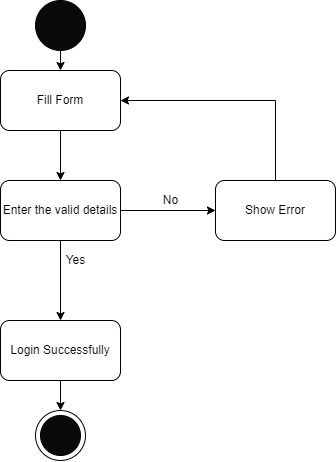
\includegraphics[scale=0.7]{./diagrams/Activity Diagram/ad-01.png}
    \caption{Activity diagram of UC-1}
    \label{fig:act-01}

\end{figure}

\textbf{Cyclomatic Complexity}

M= E-N + 2(P)

E= number of edges

N= number of nodes

P= number of paths

E= 6,
N= 6,
P= 1,

M= 6-6+2(1)= 2

\begin{figure}[H]
    \centering
    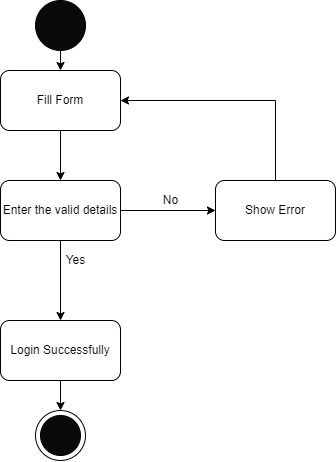
\includegraphics[scale=0.7]{./diagrams/Activity Diagram/ad-02.png}
    \caption{Activity diagram of UC-2}
    \label{fig:act-02}

\end{figure}

\textbf{Cyclomatic Complexity}

M= E-N + 2(P)

E= number of edges

N= number of nodes

P= number of paths

E= 6,
N= 6,
P= 1,

M= 6-6+2(1)= 2

\begin{figure}[H]
    \centering
    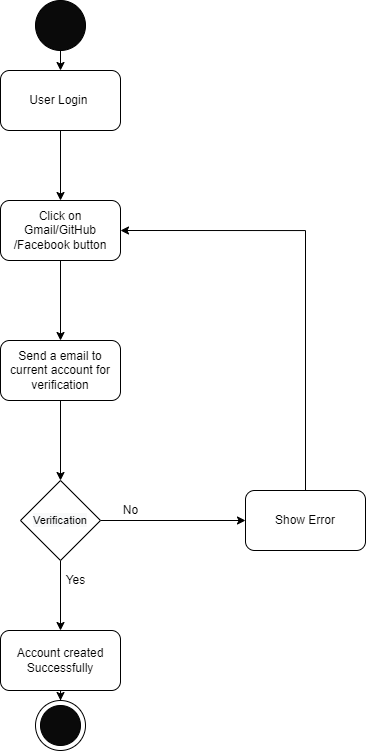
\includegraphics[scale=0.7]{./diagrams/Activity Diagram/ad-03.png}
    \caption{Activity diagram of UC-3}
    \label{fig:act-03}

\end{figure}

\textbf{Cyclomatic Complexity}

M= E+N + 2(P)

E= number of edges

N= number of nodes

P= number of paths

E= 8,
N= 8,
P= 1,

M= 8-8+2(1)= 2

\begin{figure}[H]
    \centering
    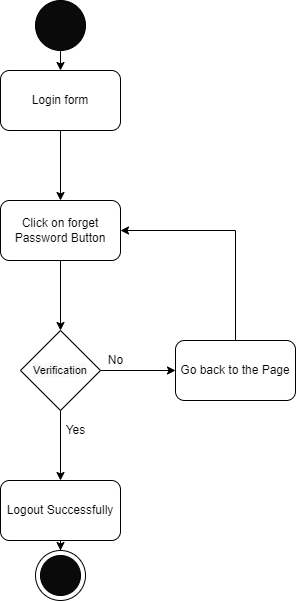
\includegraphics[scale=0.7]{./diagrams/Activity Diagram/ad-04.png}
    \caption{Activity diagram of UC-4}
    \label{fig:act-04}

\end{figure}

\textbf{Cyclomatic Complexity}

M= E+N + 2(P)

E= number of edges

N= number of nodes

P= number of paths

E= 7,
N= 7,
P= 1,

M= 7-7+2(1)= 2

\begin{figure}[H]
    \centering
    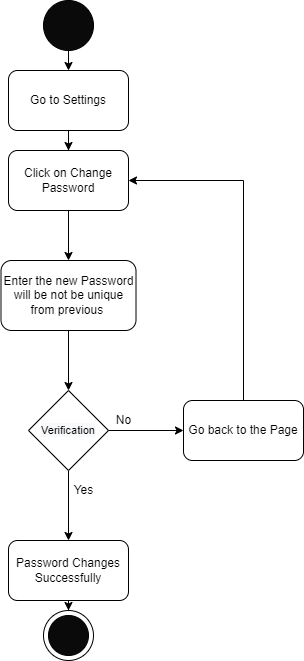
\includegraphics[scale=0.7]{./diagrams/Activity Diagram/ad-05.png}
    \caption{Activity diagram of UC-7}
    \label{fig:act-05}

\end{figure}


\textbf{Cyclomatic Complexity}

M= E+N + 2(P)

E= number of edges

N= number of nodes

P= number of paths

E= 8,
N= 8,
P= 1,

M= 8-8+2(1)= 2

\begin{figure}[H]
    \centering
    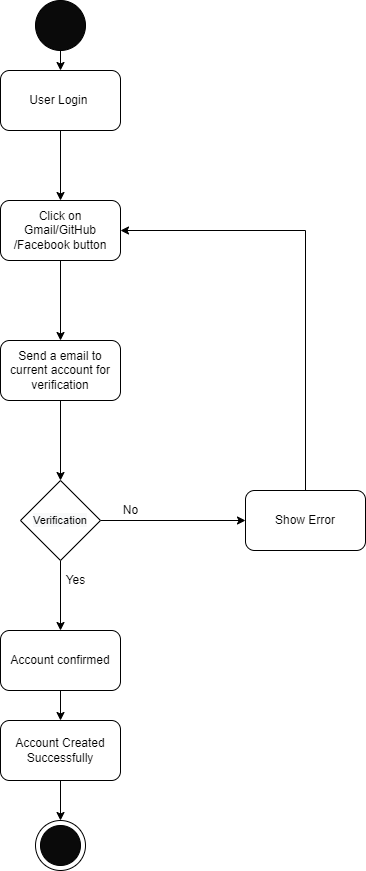
\includegraphics[scale=0.6]{./diagrams/Activity Diagram/ad-06.png}
    \caption{Activity diagram of UC-6}
    \label{fig:act-06}

\end{figure}


\textbf{Cyclomatic Complexity}
\textbf{Cyclomatic Complexity}

M= E+N + 2(P)

E= number of edges

N= number of nodes

P= number of paths

E= 9,
N= 9,
P= 1,

M= 9-9+2(1)= 2

\begin{figure}[H]
    \centering
    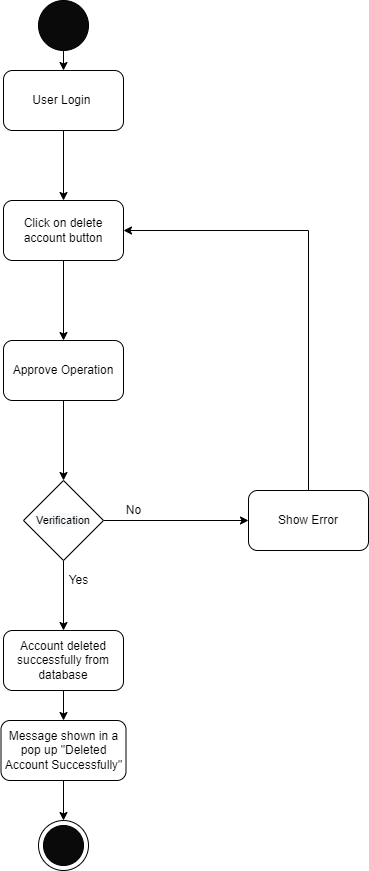
\includegraphics[scale=0.6]{./diagrams/Activity Diagram/ad-07.png}
    \caption{Activity diagram of UC-7}
    \label{fig:act-07}

\end{figure}


\textbf{Cyclomatic Complexity}

M= E+N + 2(P)

E= number of edges

N= number of nodes

P= number of paths

E= 9,
N= 9,
P= 1,

M= 9-9+2(1)= 2

\begin{figure}[H]
    \centering
    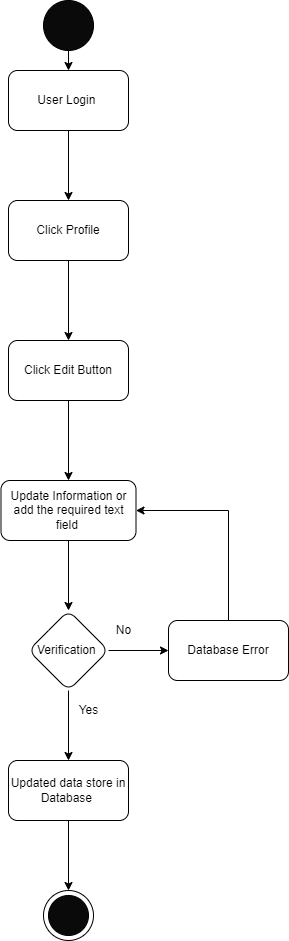
\includegraphics[scale=0.6]{./diagrams/Activity Diagram/ad-08.png}
    \caption{Activity diagram of UC-8}
    \label{fig:act-08}

\end{figure}


\textbf{Cyclomatic Complexity}


M= E+N + 2(P)

E= number of edges

N= number of nodes

P= number of paths

E= 9,
N= 9,
P= 1,

M= 9-9+2(1)= 2

\begin{figure}[H]
    \centering
    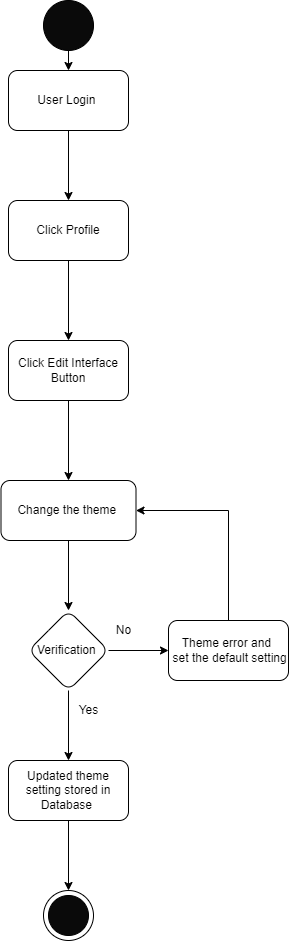
\includegraphics[scale=0.6]{./diagrams/Activity Diagram/ad-09.png}
    \caption{Activity diagram of UC-9}
    \label{fig:act-09}

\end{figure}


\textbf{Cyclomatic Complexity}

M= E+N + 2(P)

E= number of edges

N= number of nodes

P= number of paths

E= 9,
N= 9,
P= 1,

M= 9-9+2(1)= 2

\begin{figure}[H]
    \centering
    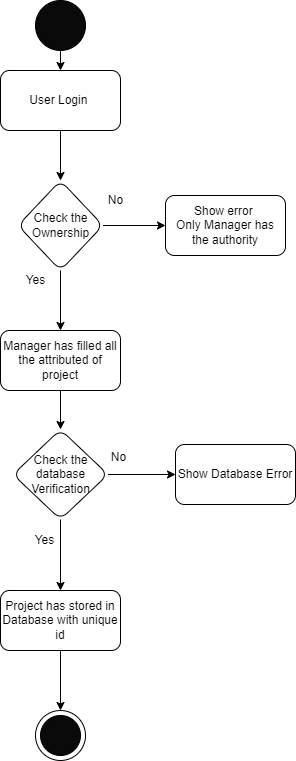
\includegraphics[scale=0.7]{./diagrams/Activity Diagram/ad-10.png}
    \caption{Activity diagram of UC-10}
    \label{fig:act-10}

\end{figure}


\textbf{Cyclomatic Complexity}
M= E+N + 2(P)

E= number of edges

N= number of nodes

P= number of paths

E= 8,
N= 9,
P= 1,

M= 8-9+2(1)= 1

\begin{figure}[H]
    \centering
    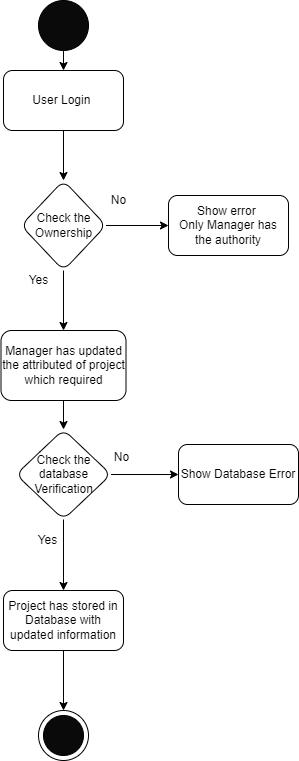
\includegraphics[scale=0.7]{./diagrams/Activity Diagram/ad-11.png}
    \caption{Activity diagram of UC-11}
    \label{fig:act-11}

\end{figure}


\textbf{Cyclomatic Complexity}

M= E+N + 2(P)

E= number of edges

N= number of nodes

P= number of paths

E= 8,
N= 9,
P= 1,

M= 8-9+2(1)= 1

\begin{figure}[H]
    \centering
    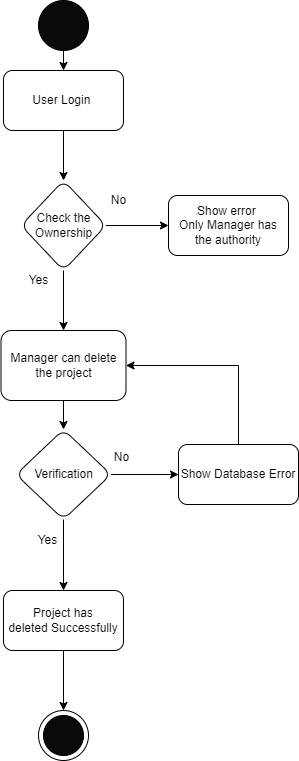
\includegraphics[scale=0.7]{./diagrams/Activity Diagram/ad-12.png}
    \caption{Activity diagram of UC-12}
    \label{fig:act-12}

\end{figure}


\textbf{Cyclomatic Complexity}

M= E+N + 2(P)

E= number of edges

N= number of nodes

P= number of paths

E= 9,
N= 9,
P= 1,

M= 9-9+2(1)= 2

\begin{figure}[H]
    \centering
    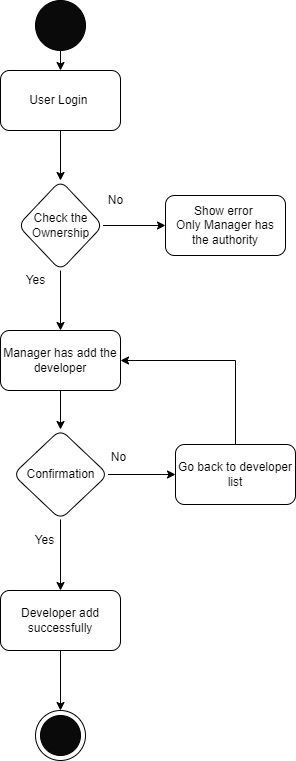
\includegraphics[scale=0.7]{./diagrams/Activity Diagram/ad-13.png}
    \caption{Activity diagram of UC-13}
    \label{fig:act-13}

\end{figure}


\textbf{Cyclomatic Complexity}

M= E+N + 2(P)

E= number of edges

N= number of nodes

P= number of paths

E= 9,
N= 9,
P= 1,

M= 9-9+2(1)= 2

\begin{figure}[H]
    \centering
    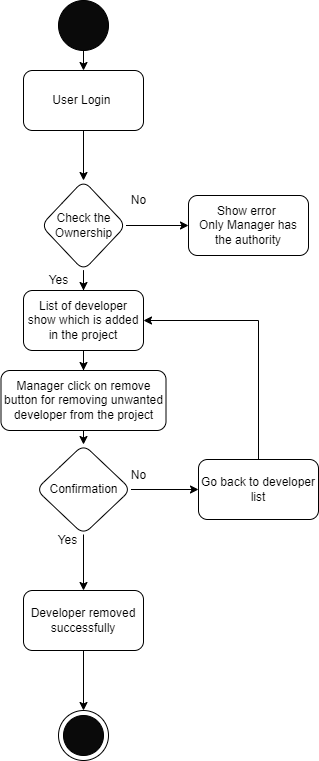
\includegraphics[scale=0.7]{./diagrams/Activity Diagram/ad-14.png}
    \caption{Activity diagram of UC-14}
    \label{fig:act-14}

\end{figure}


\textbf{Cyclomatic Complexity}

M= E+N + 2(P)

E= number of edges

N= number of nodes

P= number of paths

E= 10,
N= 10,
P= 1,

M= 10-10+2(1)= 2

\begin{figure}[H]
    \centering
    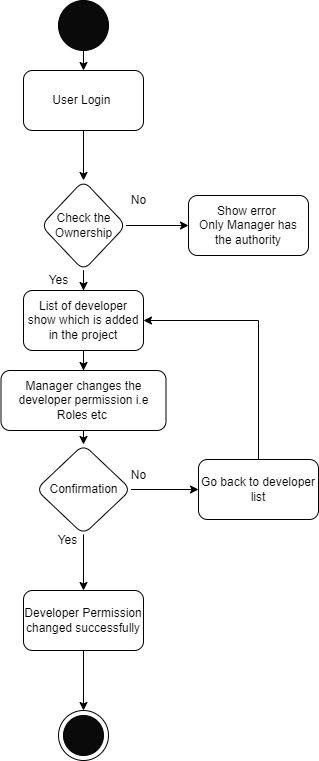
\includegraphics[scale=0.7]{./diagrams/Activity Diagram/ad-15.png}
    \caption{Activity diagram of UC-15}
    \label{fig:act-15}

\end{figure}


\textbf{Cyclomatic Complexity}

M= E+N + 2(P)

E= number of edges

N= number of nodes

P= number of paths

E= 10,
N= 10,
P= 1,

M= 10-10+2(1)= 2

\begin{figure}[H]
    \centering
    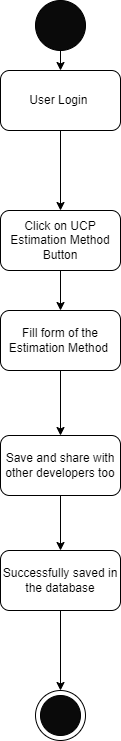
\includegraphics[scale=0.7]{./diagrams/Activity Diagram/ad-16.png}
    \caption{Activity diagram of UC-16}
    \label{fig:act-16}

\end{figure}


\textbf{Cyclomatic Complexity}

M= E+N + 2(P)

E= number of edges

N= number of nodes

P= number of paths

E= 6,
N= 7,
P= 1,

M= 6-7+2(1)= 1

\begin{figure}[H]
    \centering
    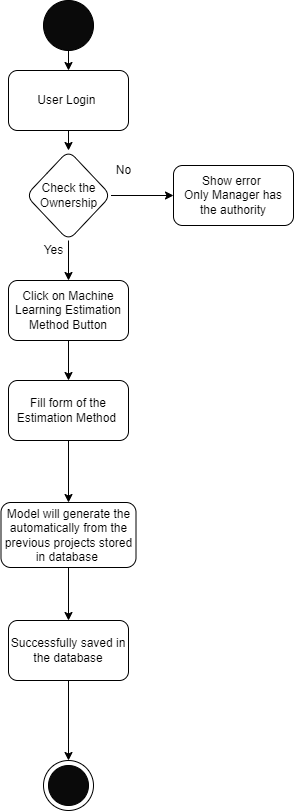
\includegraphics[scale=0.7]{./diagrams/Activity Diagram/ad-17.png}
    \caption{Activity diagram of UC-17}
    \label{fig:act-17}

\end{figure}

\textbf{Cyclomatic Complexity}

M= E+N + 2(P)

E= number of edges

N= number of nodes

P= number of paths

E= 8,
N= 9,
P= 1,

M= 8-9+2(1)= 1

\begin{figure}[H]
    \centering
    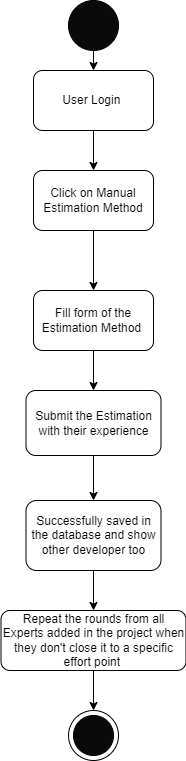
\includegraphics[scale=0.7]{./diagrams/Activity Diagram/ad-18.png}
    \caption{Activity diagram of UC-18}
    \label{fig:act-18}

\end{figure}


\textbf{Cyclomatic Complexity}

M= E+N + 2(P)

E= number of edges

N= number of nodes

P= number of paths

E= 7,
N= 8,
P= 1,

M= 7-8+2(1)= 1

\begin{figure}[H]
    \centering
    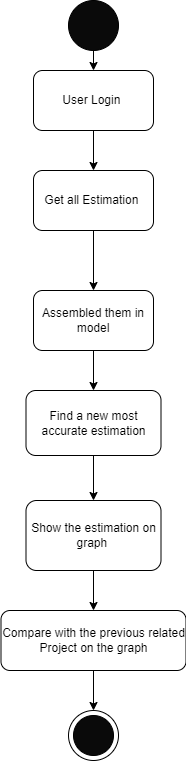
\includegraphics[scale=0.7]{./diagrams/Activity Diagram/ad-19.png}
    \caption{Activity diagram of UC-19}
    \label{fig:act-19}

\end{figure}

\textbf{Cyclomatic Complexity}

M= E+N + 2(P)

E= number of edges

N= number of nodes

P= number of paths

E= 7,
N= 8,
P= 1,

M= 7-8+2(1)= 1

\begin{figure}[H]
    \centering
    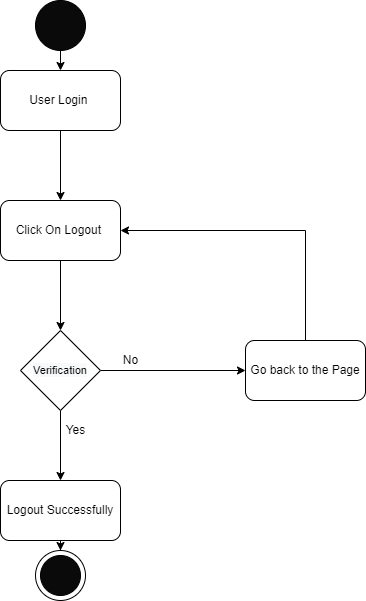
\includegraphics[scale=0.7]{./diagrams/Activity Diagram/ad-20.png}
    \caption{Activity diagram of UC-20}
    \label{fig:act-20}

\end{figure}


\textbf{Cyclomatic Complexity}

M= E+N + 2(P)

E= number of edges

N= number of nodes

P= number of paths

E= 7,   N= 7,   P= 1,

M= 7-7+2(1)= 2
